% !TEX TS-program = pdflatex
% !TEX encoding = UTF-8 Unicode

% This is a simple template for a LaTeX document using the "article" class.
% See "book", "report", "letter" for other types of document.

\documentclass[11pt]{article} % use larger type; default would be 10pt

\usepackage[utf8]{inputenc} % set input encoding (not needed with XeLaTeX)

%%% Examples of Article customizations
% These packages are optional, depending whether you want the features they provide.
% See the LaTeX Companion or other references for full information.

%%% PAGE DIMENSIONS
\usepackage{geometry} % to change the page dimensions
\geometry{a4paper} % or letterpaper (US) or a5paper or....
% \geometry{margin=2in} % for example, change the margins to 2 inches all round
% \geometry{landscape} % set up the page for landscape
%   read geometry.pdf for detailed page layout information

\usepackage{graphicx} % support the \includegraphics command and options

% \usepackage[parfill]{parskip} % Activate to begin paragraphs with an empty line rather than an indent

%%% PACKAGES
\usepackage{booktabs} % for much better looking tables
\usepackage{array} % for better arrays (eg matrices) in maths
\usepackage{paralist} % very flexible & customisable lists (eg. enumerate/itemize, etc.)
\usepackage{verbatim} % adds environment for commenting out blocks of text & for better verbatim
\usepackage{subfig} % make it possible to include more than one captioned figure/table in a single float
% These packages are all incorporated in the memoir class to one degree or another...

\usepackage[export]{adjustbox}
\usepackage{graphicx}
\usepackage{amssymb}
\usepackage{hyperref}
\hypersetup{
    colorlinks=true,
    linkcolor=blue,
    filecolor=magenta,      
    urlcolor=cyan,
}
\usepackage{relsize}
\usepackage[utf8]{inputenc}
\usepackage[greek,english]{babel}
\usepackage{alphabeta}
\usepackage{amsmath}
\usepackage{physics}
\usepackage{amsfonts}
\usepackage{nccmath}








%%% HEADERS & FOOTERS
\usepackage{fancyhdr} % This should be set AFTER setting up the page geometry
\pagestyle{fancy} % options: empty , plain , fancy
\renewcommand{\headrulewidth}{0pt} % customise the layout...
\lhead{}\chead{}\rhead{}
\lfoot{}\cfoot{\thepage}\rfoot{}

%%% SECTION TITLE APPEARANCE
\usepackage{sectsty}
\allsectionsfont{\sffamily\mdseries\upshape} % (See the fntguide.pdf for font help)
% (This matches ConTeXt defaults)

%%% ToC (table of contents) APPEARANCE
\usepackage[nottoc,notlof,notlot]{tocbibind} % Put the bibliography in the ToC
\usepackage[titles,subfigure]{tocloft} % Alter the style of the Table of Contents
\renewcommand{\cftsecfont}{\rmfamily\mdseries\upshape}
\renewcommand{\cftsecpagefont}{\rmfamily\mdseries\upshape} % No bold!

%%% END Article customizations

%%% The "real" document content comes below...


\title{
    {
\includegraphics[width=0.2\textwidth]{emp.jpg}}\\
    {\large  Εθνικό Μετσόβιο Πολυτεχνείο}\\
    {\large  Τμήμα Χημικών Μηχανικών}\\
    {Ανάπτυξη Μεθοδολογίας Αυτόματης Ρύθμισης Συστημάτων με Εκπαίδευση Νευρωνικών Δικτύων Βάθους}\\
}
\author{Στεφανής Μιχαήλ}
\date{2 Ιουλίου 2018}

\begin{document}
\maketitle
\newpage

\tableofcontents
\listoffigures

\newpage

\[ 
\ r(s,α,s') = \left\{
\begin{array}{ll}
      c & , \abs{y^{i} - (y_{set})^{i}} \leq ε  \forall i \\
      -\sum_{i=1}^{n} \abs{y^{i} - (y_{set})^{i}} & otherwise \\
\end{array} 
\right. 
\]

$L(W_c) = \mathbb{E}[(r + \gamma Q_t - Q(s,α,W_c))^2]$ \\

$\pdv{L(W_c)}{W_c} = \mathbb{E}[(r + \gamma Q_t - Q(s,α,W_c))\pdv{Q(s,α,W_c}{W_c}]$ \\

$\pdv{J(W_α)}{W_α} = \mathbb{E}[\pdv{Q(s,α,W_c)}{α} \pdv{π(s,W_α)}{W_α}]$ \\

$G(s) = \frac{Y(s)}{U(s)} = \frac{0.05s}{1-0.6s}$

$\nabla_p \leftarrow \nabla_p$

\[ 
\left\{
\begin{array}{ll}
      \frac{p_{max}-p}{p_{max}-p_{min}} & άν ο \nabla_p δηλωνει αύξηση \\
      \frac{p-p_{min}}{p_{max}-p_{min}} & otherwise \\
\end{array} 
\right. 
\] 


Ένας τεράστιος αριθμός σύγχρονων τεχνολογικών και επιστημονικών εφαρμογών βασίζονται στην ικανότητα των νευρωνικών δικτύων να συσχετίζουν σχεδόν κάθε είδους δεδομένων εισόδου με μία επιθυμητή έξοδο, δηλαδή στο να βρίσκουν μία συνάρτηση που να τα συσχετίζει. Πιο σωστά, τα νευρωνικά δίκτυα δρούν ως \textit{συναρτησιακοί προσεγγιστές} (function approximators), με την έννοια ότι μπορούν να "πλησιάσουν" μια επιθυμητή συνάρτηση με πολύ μεγάλη ακρίβεια. Πώς όμως μπορεί κανείς να είναι σίγουρος ότι η αρχιτεκτονική των νευρωνικών δικτύων θα είναι όντως ικανή να επιλύσει το εκάστοτε πρόβλημα; Στα πλαίσια των πραγματικών εφαρμογών οι συναρτήσεις που επιθυμούμε να προσεγγίσουμε μπορεί να είναι πολύ περίπλοκες ή ακόμη και να μην έχουν σαφή (explicit) μορφή. \\

Στο ερώτημα αυτό δίνει μία πολύ ικανοποιητική απάντηση το πανίσχυρο \textit{Θεώρημα Καθολικής Προσέγγισης για Νευρωνικά Δίκτυα} (Universal Approximation Theorem for Neural Networks). Το θεώρημα αυτό έχει μία πολύ καθορισμένη και αυστηρή Μαθηματική θεμελίωση.  Μας λέει πως μπορούμε να προσεγγίσουμε όσο καλά θέλουμε μια συνεχή συνάρτηση ορισμένη σε ένα συμπαγές σύνολο με ένα προωθητικό νευρωνικό δίκτυο που περιέχει \textit{μονάχα ένα κρυφό στρώμα} το οποίο θα αποτελείται από \textit{πεπερασμένους νευρώνες}. Η απόδειξη του θεωρήματος δεν είναι απλή και χρησιμοποιεί πολλά βαριά εργαλεία της συναρτησιακής ανάλυσης και της θεωρίας μέτρου, όπως το θεώρημα Hahn-Banach και το Θεώρημα Κυρίαρχης Σύγκλισης. Παρόλα αυτά μας εξασφαλίζει την αδιαμφησβήτητη ικανότητα των νευρωνικών δικτύων να μας παρέχουν, με μία σχετικά απλή αρχιτεκτονική, οποιαδήποτε ομοιόμορφα συνεχή συνάρτηση θέλουμε. Πρίν δοθεί η πλήρης Μαθηματική περιγραφή του θεωρήματος θα χρειαστούμε μερικούς ορισμούς. \\ 

\textbf{Ορισμός}: Μία συνάρτηση \sigma : $\mathbb{R}$ $\rightarrow$ $\mathbb{R}$ θα λέγεται \textit{σιγμοειδής} (sigmoidal) αν είναι γνήσια μονότονη και ικανοποιεί: 

\[ 
\ \sigma(t) = \left\{
\begin{array}{ll}
      α & , t \rightarrow +\infty \\
      β & , t \rightarrow -\infty \\
\end{array} 
\right. 
\]
για κάποιους πραγματικούς αριθμούς α και β. Δηλαδή μία σιγμοειδής συνάρτηση είναι φραγμένη.  Στις περισσότερες εφαρμογές και πολύ συνχά στην βιβλιογραφία οι σιγμοειδείς συναρτήσεις επιλέγονται με τέτοιο τρόπο ώστε να είναι κανονικοποιημένες, δηλαδή α = 1 και β = 0 ή α = 1 και β = -1. \\

 Παραδείγματα σιγμοειδών συναρτήσεων αποτελούν οι εξής συναρτήσεις : \\
\begin{itemize}
  \item \textit{Λογιστική Συνάρτηση}, \sigma(x) = $\frac{1}{1 + e^{-x}}$ 
  \item \textit{Υπερβολική Εφαπτομένη} \sigma(x) = $\frac{e^x - e^{-x}}{e^x + e^{-x}}$
  \item \textit{Συνάρτηση Σφάλματος} \sigma(x) = $\displaystyle \frac{2}{\sqrt{\pi}} \int_{0}^{x} e^{-t^2} dt$
\end{itemize}


\textbf{Ορισμός}:Έστω $Ι_n$ ο μοναδιαίος n-διάστατος κύβος. Μία συνάρτηση $\sigma$ θα λέγεται \textit{μεροληπτική} (discriminatory) εάν ισχύει η συναπαγωγή: \\
\begin{equation}
 \displaystyle \int_{I_n} \sigma(\textbf{w}_i ^\intercal \mathbf{x} + b_i) d\mu(x) = 0 \Rightarrow \mu(x) = 0  
\end{equation} 

$\forall$ $\textbf{w}_i$ $\in$   $\mathbb{R}^d$ , $b_i$ $\in$ $\mathbb{R}$, $\mu$ $\in$ $M(I_n)$.\\

Η συνάρτηση \mu \textbf(x) αποτελεί ένα κάπως τεχνικό εργαλείο και καλείται \textit{μέτρο}. Είναι μια συνάρτηση που ορίζεται σε ένα σύνολο και μας επιτρέπει να αντιστοιχίσουμε σε κάθε υποσύνολο του συνόλου αυτού έναν θετικό πραγματικό αριθμό, ο οποίος διαισθητικά μπορεί να ερμηνευθεί ώς το \textit{μέγεθος} του υποσυνόλου αυτού. Ο παραπάνω ορισμός μας λέει πως μία μεροληπτική συνάρτηση μπορεί να δράσει \textit{μη-καταστρεπτικά} σε έναν γραμμικό συνδυασμό πραγματικών αριθμών με εξαίρεση ένα υποσύνολο που έχει μέτρο ίσο με το μηδέν (\mu = 0). Διαισθητικά, ένα σύνολο έχει μέτρο ίσο με το μηδέν όταν ο πληθάριθμός του είναι πεπερασμένος. Συνεπώς μια μεροληπτική συνάρτηση επιτρέπει στην πληροφορία να περάσει από τον έναν νευρώνα στον επόμενο χωρίς να χαθεί η πληροφορία της εισόδου.\\

Έστω Α $\subset$ $\mathbb{R}$ ένα συμπαγές σύνολο (κλειστό και φραγμένο). Θα συμβολίζουμε το σύνολο των συνεχών, μεροληπτικών και μη γραμμικών σιγμοειδών συναρτήσεων ορισμένες στο Α με παραμέτρους α και β ώς \textbf{Sig(A,α,β)}. Επειδή το Α είναι συμπαγές και οι συναρτήσεις συνεχείς σημαίνει ότι το Sig(A,α,β) αποτελείται από ομοιόμορφα συνεχείς -και άρα ολοκληρώσιμες- συναρτήσεις. \\

Παρακάτω δίνουμε έναν μαθηματικό ορισμό ενός νευρωνικού δικτύου με ένα μόνο κρυφό στρώμα: \\

\textbf{Ορισμός}: Ένα \textit{νευρωνικό δίκτυο} $Ν$ νευρώνων (ή κόμβων) διατεταγμένων σε ένα μόνο κρυφό στρώμα είναι μία συνάρτηση $\Psi : \mathbb{R}^n \rightarrow \mathbb{R}$ που δίνεται από την σχέση:
\begin{equation}
 \displaystyle \Psi(\textbf{x}) = \sum_{i=1}^{N} u_i \sigma(\textbf{w}_i ^ \intercal \textbf{x} + b_i)
\end{equation}

όπου  $\textbf{w}_i,\textbf{x}  \in \mathbb{R}^n, u_i,b_i \in \mathbb{R}$ και \sigma $\in$ Sig($I_n$,α,β). Το σύνολο των νευρωνικών δικτύων της παραπάνω μορφής που αποτελούνται από  θα συμβολίζεται με $\aleph.$ \\

\textbf{Θεώρημα} (Καθολικής Προσέγγισης για Νευρωνικά Δίκτυα): Έστω $\sigma : \mathbb{R} \rightarrow \mathbb{R}$  με  \sigma  $\in$ Sig($I_n$,α,β) και C($I_n$) το σύνολο των συνεχών συναρτήσεων στο $Ι_n$ (ή σε οποιοδήποτε συμπαγές υποσύνολο του $\mathbb{R}^n$ . Τότε το σύνολο $\aleph$ είναι \textit{πυκνό} στο C($I_n$). Δηλαδή για κάθε $\epsilon > 0$ και κάθε συνάρτηση $f$ $\in$ C($I_n$) υπάρχει ένα νευρωνικό δίκτυο της μορφής (2) τέτοιο ώστε: \\
 \begin{align*}
\abs{\Psi(x) - f(x)} < \epsilon 
\end{align*}
$\forall x \in I_n$. \\

Από το παραπάνω κεντρικό θεώρημα φαίνεται ότι η αρχιτεκτονική των νευρωνικών δικτύων είναι παραπάνω από ικανή για να δράσει ώς συναρτησιακός προσεγγιστής. Ένα δίκτυο με ένα μόνο κρυφό στρώμα αρκεί για να μας εξασφαλίσει όλες τις συνεχείς και φραγμένες συναρτήσεις, πόσο μάλλον ένα "βαθύτερο" δίκτυο με παραπάνω κρυφά στρώματα. \\

\begin{table}[h!]
\centering
\begin{tabular}{|p{0.3cm}|p{6cm}|}
\hline
\multicolumn{2}{|c|}{\textbf{Αλγόριθμος Εκμάθησης}} \\
\hline
1 & Αρχικοποίηση Δικτύων Δράστη και Κριτή \\
\hline
2 & Αρχικοποίηση Δικτύων Στόχου Δράστη και Κριτή\\
\hline
3 & Αρχικοποίηση Μνήμης Αναπαραγωγής \\
\hline
4  & \textbf{For episode = 1 to E do}: \\
\hline
5  & Επαναφορά (reset) θορύβου κατά Ornstein-Uhlenbeck $\aleph_t$  \\
\hline
6 & Τυχαίος Ορισμός τελική κατάστασης $y_{set}$  \\
\hline
7 & \textbf{For time step = 1 to T do} \\
\hline
8 & Παρατήρηση τρέχουσας κατάστασης s $\leftarrow [y_t, y_{set}]$ \\
\hline
9 & Εκτέλεση Δράσης $α = u_t = \pi(s, W_α) + \aleph_t $\\
\hline
10 & Παρατήρηση επόμενης κατάστασης $s' = [y_{t+1}, y_{set}]$\\
\hline
11 & Λήψη αμοιβής $r_t$\\
\hline
12 & Αποθήκευση της τετράδας $[s, α, s', r]$ στην Μνήμη Αναπαραγωγής\\
\hline
13 & Λήψη τυχαίας παρτίδας $n$ τετράδων από την Μνήμη Αναπαραγωγής\\
\hline
14 & \textbf{For minibatch = 1 to $N$ do}: \\
\hline
15 & Υπολογισμός της ποσότητας $\phi_i = r_i + Q_t ^ i$ για κάθε τετράδα της παρτίδας\\
\hline
16 & Επικαιροποίηση του Κριτή : $W_α \leftarrow W_α + \alpha \pdv{L(W_c)}{W_c}$\\
\hline
17 & Υπολογισμός του $\nabla _p ^ i = \pdv{Q(s^i, α^i, W_c)}{α^i}$\\
\hline
18 & Επικαιροποίηση του Δράστη : $W_c \leftarrow W_c + \alpha \pdv{J(W_α)}{W_α}$\\
\hline
19 & \textbf{If $time step = 0 \mod(D)$ do}:\\
\hline
20 & Επικαιροποίηση Δικτύου Στόχου Κριτή: $W_α ^ t \leftarrow \tau W_α + (1-\tau)W_α ^t$\\
\hline
21 & Επικαιροποίηση Δικτύου Στόχου Δράστη:  $W_c ^ t \leftarrow \tau W_c + (1-\tau)W_c ^t$\\
\hline
22 & \textbf{endfor}\\
\hline
23 & \textbf{endfor}\\
\hline
\end{tabular}
\caption{Αλγόριθμος εκμάθησης μεθοδολογίας DDPG}
\label{table:1}
\end{table}

\section{Αρχιτεκτονική Νευρωνικών Δικτύων}

\subsection{Συναρτήσεις Ενεργοποίησης}

Οι συναρτήσεις ενεργοποίησης είναι ο τρόπος με τον οποίο η πληροφορία των σημάτων εισόδου περνούν από τον έναν νευρώνα στον επόμενο. Σηματοδοτούν δηλαδή πότε ένας νευρώνας θα "ενεργοποιηθεί" και θα μεταβιβάσει την εκάστοτε πληροφορία. Υπάρχουν πολλές υποψήφιες επιλογές συναρτήσεων ενεργοποίησης και η επιλογή της "καταλληλότερης" συνάρτησης για τον κάθε νευρώνα (η συνηθέστερα για το κάθε κρυφό στρώμα) είναι ως επί το πλείστον εμπειρική και αποτελεί πηγή πολλών ερευνητικών δυνατοτήτων. Για να καταλάβουμε τί είδους συναρτήσεις είναι κατάλληλες για την μεταφορά πληροφορίας μεταξύ των νευρώνων μπορούμε να ξεκινήσουμε μελετώντας ποιες συναρτήσεις \textit{δεν είναι κατάλληληλες} για αυτόν τον σκοπό.\\

Η μελέτη των συναρτήσεων ενεργοποίησης ξεκίνησε με την εξής απλή σκέψη: Εφόσον ένας νευρώνας είτε θα μεταβιβάσει είτε δεν θα μεταβιβάσει την πληροφορία στον επόμενο νευρώνα, τι πιο φυσικό από το να χρησιμοποιήσουμε την \textit{βηματική συνάρτηση} (step function): 

\[ 
\ \sigma(t) = \left\{
\begin{array}{ll}
      1 & , x > 0 \\
      0 & , x < 0 \\
\end{array} 
\right. 
\]

Παρόλο που η παραπάνω συνάρτηση φαίνεται διαισθητικά σωστή, στην πραγματικότητα εμφανίζει πολύ άσχημα αποτελέσματα στην πράξη της εκπαίδευσης των δικτύων. Αυτό οφείλεται στο γεγονός ότι ο ορισμός της παραπάνω συνάρτησης θα επιτρέψει στον νευρώνα είτε να μεταδώσει πλήρως την πληροφορία του είτε καθόλου, ενεργεί δηλαδή με δυαδικό τρόπο. Στην πράξη παρόλα αυτά μία καλή εκπαίδευση θα πρέπει να περιλαμβάνει και "ποσοστά μετάδοσης" πληροφορίας επειδή με αυτόν τον τρόπο η εκπαίδευση του δικτύου \\

Συνεπώς θα πρέπει να επιλέξουμε μία συνάρτηση που να δίνει και ενδιάμεσες τιμές ενεργοποίησης. Η πρώτη σκέψη είναι μία γραμμική συνάρτηση:
\begin{align*}
\sigma (x) = \alpha x
\end{align*}

Μια συνάρτηση τέτοιας μορφής μπορεί να δώσει όντως μια μεγάλη ποικιλία τιμών ενεργοποίησης, οι οποίες τιμές είναι ανάλογες της εκάστοτε εισόδου. Παρόλα αυτά οι γραμμικές συναρτήσεις έχουν δύο σοβαρά μειονεκτήματα. Το πρώτο είναι το γεγονός ότι έχουν \textit{σταθερή βαθμίδα} (ή \textit{κλίση}). Αυτό σημαίνει ότι αν υπάρχει σφάλμα στην πρόβλεψη, δηλαδή η έξοδος του νευρωνικού δικτύου διαφέρει από την επιθυμητή τιμή, τότε η διόρθωση και οι αλλαγές που θα γίνονται με την προς-τα-πίσω μετάδοση θα είναι σταθερές και δεν θα εξαρτώνται από το σφάλμα αυτό. Το δεύτερο μειονέκτημα δεν είναι τόσο προφανές. Αν όλες οι συναρτήσεις ενεργοποίησης επιλεγούν γραμμικές τότε η τελική έξοδος του νευρωνικού δικτύου θα είναι και αυτή μία γραμμική συνάρτηση της εισόδου. Στην ουσία το σύνολο του νευρωνικού δικτύου (που μπορεί να περιέχει μέχρι και δεκάδες κρυφά στρώματα!) θα είναι ισοδύναμο με ένα νευρωνικό δίκτυο με ένα μόνο κρυφό στρώμα, εφόσον η σύνθεση γραμμικών συναρτήσεων είναι μία επίσης γραμμική συνάρτηση. Αυτό στην πράξη σημαίνει χειρότερη εκπαίδευση.\\

Το επόμενο βήμα δεν είναι ιδιαίτερα προφανές. Χρειαζόμαστε μία συνάρτηση που να έχει τουλάχιστον τις εξής ιδιότητες:
\begin{itemize}
  \item Μη-γραμμική
  \item Φραγμένη (προτιμέστερα μεταξύ του 0 και του 1, χωρίς να έχει ιδιαίτερη σημασία)
  \item Να είναι τουλάχιστον μια φορά συνεχώς παραγωγίσιμη 
\end{itemize}

Μία πολύ καλή υποψήφια συνάρτηση είναι η λεγόμενη \textit{λογιστική συνάρτηση}:
\begin{align*}
\sigma(x) = \frac{1}{1+e^{-x}}
\end{align*}

\begin{figure}[h]
    \centering
    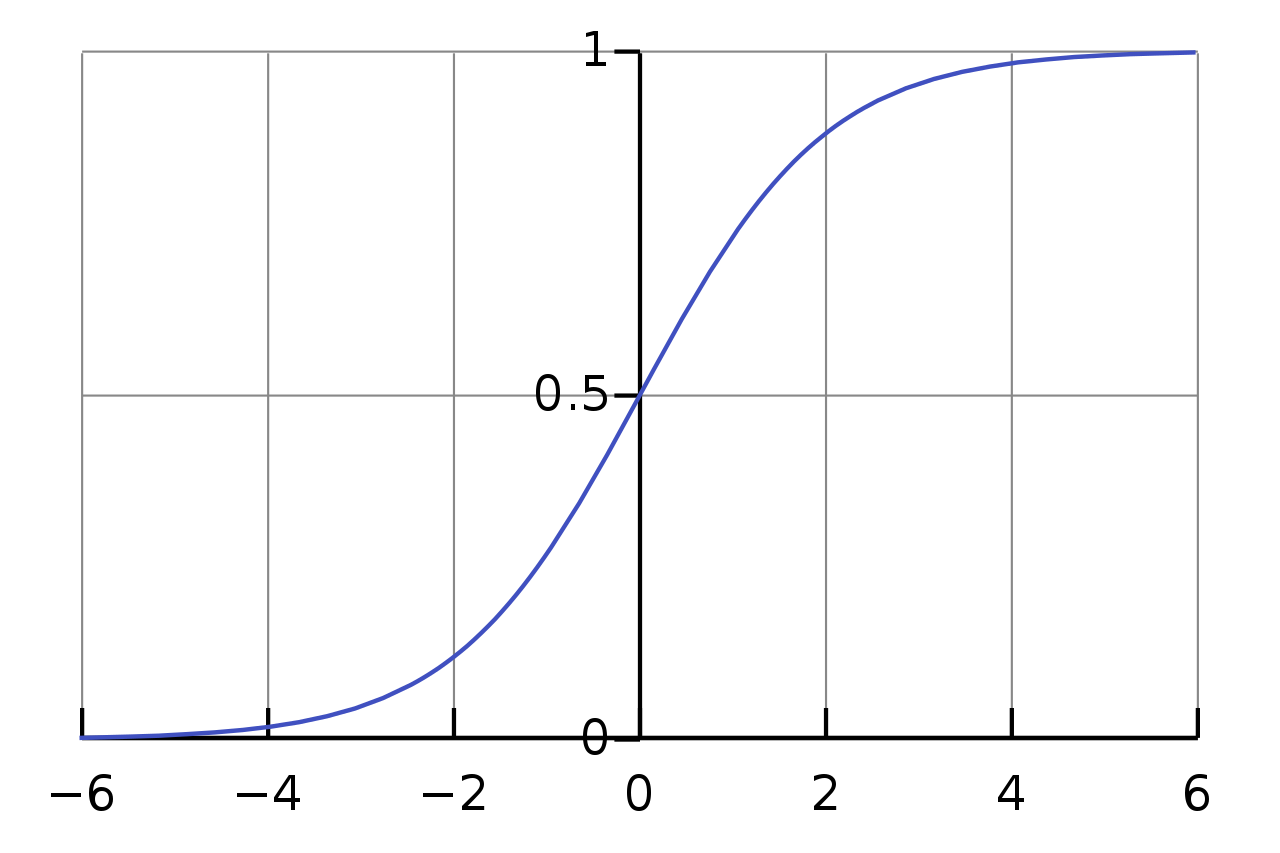
\includegraphics[width=0.6\textwidth]{logcurve}
    \caption{Γραφική παράσταση της λογιστικής συνάρτησης}
    \label{fig:logistic curve}
\end{figure}

Η παραπάνω συνάρτηση έχει όλες τις παραπάνω επιθυμητές ιδιότητες συν άλλη μία η οποία δεν είναι άμεσα προφανής. H λογιστική συνάρτηση έχει κλίση που δίνεται από τον τύπο:
\begin{align*}
\nabla \sigma(x) = \frac{e^x}{(e^x + 1)^2}
\end{align*}

 Στο διάστημα [-2,2] η κλίση της λογιστικής συνάρτησης είναι αρκετά μεγάλη, όπως φαίνεται και από την γραφική της παράσταση. Μεγάλη κλίση σημαίνει πως μικρές μεταβολές των μεταβλητών εισόδου (μικρά Δx) οδηγούν σε μεγάλες μεταβολές των μεταβλητών εξόδου. Υπάρχει δηλαδή αρκετά μεγάλη ευαισθησία σε μικρές διαταραχές του σήματος που εισέρχεται στον νευρώνα και αυτό συνεπάγεται πιο αποδοτική εκπαίδευση με την χρήση της προς-τα-πίσω μετάδοσης. \\

Η λογιστική συνάρτηση είναι όντως μία από τις ευρέως χρησιμοποιούμενες συναρτήσεις ενεργοποίησης στην τεχνολογία των νευρωνικών δικτύων λόγω των προαναφερθέντων ιδιοτήτων της. Στο σημείο αυτό όμως θα πρέπει να αναφερθεί και το μοναδικό μειονέκτημα της εν λόγω συνάρτησης που οφείλεται στην ίδια την φύση της. Παρατηρούμε από την παραπάνω γραφική παράσταση ότι στο σύνολο $[-\infty,-2] \cup [2, +\infty]$ η κλίση της λογιστικής συνάρτησης πρακτικά μηδενίζεται (η συνάρτηση τείνει να γίνει οριζόντια). Παρουσιάζεται δηλαδή το φαινόμενο των \textit{εξαφανισμένων βαθμίδων} (vanishing gradients). Πολύ μικρές βαθμίδες στα διαστήματα αυτά σημαίνει πως μόλις η εκπαίδευση μας οδηγήσει στα "άκρα" της συνάρτησης τότε η εκπαίδευση επιβραδύνεται με πολύ μεγάλο ρυθμό και πρακτικά σταματά.\\

Το επόμενο βήμα αποτελεί μία βελτίωση της λογιστικής συνάρτησης και ονομάζεται \textit{υπερβολική εφαπτομένη}:
\begin{align*}
\sigma(x) = \tanh{x} = \frac{e^x - e^{-x}}{e^x + e^{-x}}
\end{align*}

\begin{figure}[h]
    \centering
    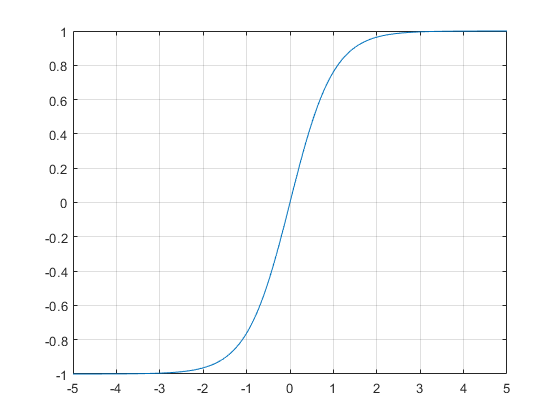
\includegraphics[width=0.6\textwidth]{tanh}
    \caption{Γραφική παράσταση της υπερβολικής εφαπτομένης}
    \label{fig:tanh curve}
\end{figure}

Συγκρίνοντας τις κλίσεις της λογιστικής συνάρτησης και της υπερβολικής εφαπτομένης παρατηρούμε ότι στο κοινό διάστημα [-2,2] η υπερβολική εφαπτομένη έχει μεγαλύτερη κλίση. Κατά τ'άλλα παρουσιάζει τα ίδια μειονεκτήματα και πλεονεκτήματα με την λογιστική συνάρτηση. Η επιλογή ανάμεσα στις δύο αυτές συναρτήσεις εξαρτάται από το πόσο μεγάλες κλίσεις θέλουμε να επιβάλλουμε στο νευρωνικό μας δίκτυο. Αποτελεί προς το παρόν θέμα κυρίως εμπειρικό και εξαρτάται από το εκάστοτε πρόβλημα.\\

Εναλλακτικές επιλογές συναρτήσεων που παρουσιάζουν παρόμοια χαρακτηριστικά με την λογιστική συνάρτηση και την υπερβολική εφαπτομένη είναι οι εξής συναρτήσεις:
\begin{gather*}
f(x) = \arctan(x) 
f(x) = \frac{x}{1+\abs{x}}
f(x) = \frac{x}{\sqrt{1+\alpha x^2}}










 





\end{document}
